%FOR PDFLATEX USE ONLY
\documentclass[a4paper,12pt]{article}

\usepackage{amssymb,amsmath} %math symbols

\usepackage[margin=2cm]{geometry} %paper geometry

\usepackage[utf8]{inputenc} %allows unicode (including russian) source file
\usepackage[russian]{babel} %docment in russian-style
\usepackage[utf8]{inputenc}
%\usepackage[unicode]{hyperref} %links inside of the text
\usepackage[pdftex]{graphicx} %includegraphics pictures
\usepackage{cmlgc} %bold text

\usepackage{array} %arrays

%\usepackage{wrapfig}
%\usepackage{array}
%\usepackage{lipsum}
%\usepackage{esvect}
%\usepackage{hyperref}

\usepackage{subfig}
%\usepackage{calc}
%\usepackage{pgfplots,tikz,circuitikz}
%\usepackage{tkz-euclide}

\begin{document}

\begin{center}
  \LARGE{Работа 3.6.1}\\[0.2cm]
  \LARGE{Спектральный анализ электрических сигналов.}\\[0.2cm]
  \large{Малиновский Владимир}\\[0.2cm]
  \normalsize{\texttt{galqiwi@galqiwi.ru}}
\end{center}

\textbf{Цель работы:} исследование спектра колебаний электрических сигналов.\\
\textbf{В работе используются:} персональный  компьютер; USB-осциллограф  АКИП-4107; функциональный генератор WaveStation2012; соединительные кабели.\\
\section*{Идея}
\subsection*{Разложение сложных сигналов на периодические колебания}
Используется разложение в сумму синусов и косинусов с различными аргументами или, как чаще его называют, \textit{разложение в ряд Фурье}.

Пусть задана функция $f(t)$, которая периодически повторяется с частотой $\Omega_1 = \dfrac{2\pi}{T}$, где $T$ --- период повторения импульсов. Её разложение в ряд Фурье имеет вид 
\begin{equation}
f(t) = \dfrac{a_0}{2} + \sum\limits_{n = 1}^{\infty}\left[a_n \cos \left(n \Omega_1t\right) + b_n \sin \left(n \Omega_1t\right)\right]
\end{equation}
или
\begin{equation}
f(t) = \dfrac{a_0}{2} + \sum\limits_{n = 1}^{\infty}A_n \cos \left(n\Omega_1t-\psi_n\right).
\end{equation}
Если сигнал чётен относительно $t=0$, в тригонометрической записи остаются только члены с косинусами. Для нечетной наоборот.

Коэффициенты определяются по формуле
\begin{equation}
\begin{array}{c}
a_n  = \dfrac{2}{T}\int\limits_{t_1}^{t_1+T}f(t)\cos\left(n \Omega_1 t\right) dt,\\
\\
b_n = \dfrac{2}{T}\int\limits_{t_1}^{t_1+T}f(t)\sin\left(n \Omega_1 t\right) dt.
\end{array}
\end{equation}
Здесь $t_1$ --- время, с которого мы начинаем отсчет.

Сравнив формулы $(1)$ и $(2)$ можно получить выражения для $A_n$  и $\psi_n$:
\begin{equation}
\begin{array}{l}
A_n = \sqrt{a_n^2+b_n^2},\\
 \psi_n = \arctan \dfrac{b_n}{a_n}.
\end{array}
\end{equation}
\subsection*{Периодическая последовательность прямоугольных импульсов}
\begin{center}
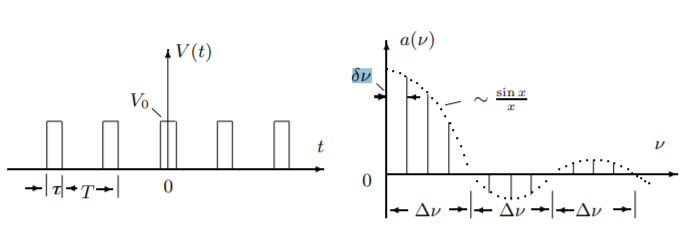
\includegraphics[scale=0.9]{2.png}
\end{center}
Введем величину: $\Omega_1 = \dfrac{2\pi}{T}$,
где $T$ --- период повторения импульсов.

Коэффициенты при косинусных составляющих будут равны
\begin{equation}
a_n = \dfrac{2}{T}\int\limits_{-\tau/2}^{\tau/2}V_0\cos\left(n\Omega_1 t\right)dt = 2V_0\dfrac{\tau}{T}\dfrac{\sin\left(n\Omega_1\tau/2\right)}{n\Omega_1\tau/2} \sim \dfrac{\sin x}{x}.
\end{equation}

Здесь $V_0$ - амплитуда сигнала.

Поскольку наша функция четная, то $b_n = 0$. 

Пусть $T$ кратно $\tau$. Тогда введем ширину спектра, равную $\Delta \omega$ --- расстояние от главного максимума до первого нуля огибающей, возникающего, как нетрудно убедиться при $n = \dfrac{2\pi}{\tau \Omega_1}$. При 
этом
\begin{equation}
\Delta \omega \tau \simeq 2\pi \Rightarrow \Delta \nu \Delta t \simeq 1.
\end{equation}
\subsection*{Периодическая последовательность цугов}
\begin{center}
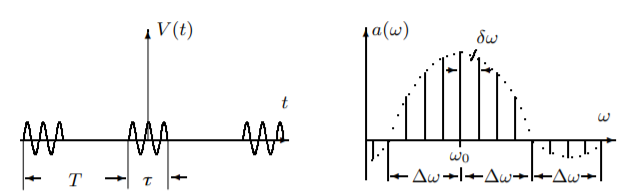
\includegraphics[scale=0.9]{3.png}
\end{center}
Возьмём цуги колебания $V_0 \cos(\omega_0 t)$ с длительностью цуга $\tau$ и периодом повторений $T$.\\
Функция $f(t)$ снова является четной относительно $t = 0$. Коэффициент при $n$-ой гармонике согласно формуле $(3)$ равен
\begin{equation}
a_n = \dfrac{2}{T}\int\limits_{-\tau/2}^{\tau/2}V_0 \cos \left(\omega_0t\right) \cdot \cos\left(n \Omega_1t\right)dt = V_0 \dfrac{\tau}{T}\left( \dfrac{\sin\left[\left(\omega_0 - n \Omega_1\right)\dfrac{\tau}{2}\right]}{\left( \omega_0 - n \Omega_1\right) \dfrac{\tau}{2}} + \dfrac{\sin\left[\left(\omega_0 + n \Omega_1\right)\dfrac{\tau}{2}\right]}{\left( \omega_0 + n \Omega_1\right) \dfrac{\tau}{2}}\right).
\end{equation}
Пусть $T$ кратно $\tau$. Тогда спектры последовательности прямоугильных сигналов и цугов аналогичны, но максимумы сдвинуты на $\omega_0$.
\subsection*{Амплитудно-модулированные колебания}
\begin{center}
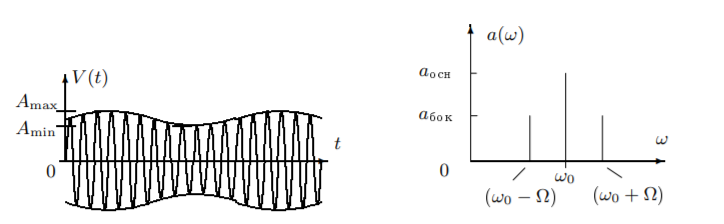
\includegraphics[scale=0.9]{4.png}
\end{center}
Рассмотрим гармонические колебания высокой частоты $\omega_0$, амплитуда которых медленно меняется по гармоническому закону с частотой $\Omega \ll \omega_0$.
\begin{equation}
f(t) = A_0 \left[1+m\cos \Omega t\right] \cos \omega_0 t.
\end{equation}
Коэффициент $m$ называется \textit{глубиной модуляции}. При $m < 1$ амплитуда меняется от минимальной $A_{min} = A_0(1-m)$ до максимальной $A_{max} = A_0(1+m)$. Глубина модуляции может быть представлена в виде
\begin{equation}
m = \dfrac{A_{max}-A_{min}}{A_{max}+A_{min}}.
\end{equation}
Простым тригонометрическим преобразованием уравнения $(8)$ можно найти спектр колебаний
\begin{equation}
f(t) = A_0 \cos \omega_0t + \dfrac{A_0m}{2} \cos \left(\omega_0 + \Omega\right)t + \dfrac{A_0m}{2}\cos\left(\omega_0 - \Omega\right)t.
\end{equation}
\section*{Метод, результаты и обработка}

\subsection*{Исследование спектра периодических последовательностей прямоугольных импульсов}
Устанавливаем прямоугольные колебания c $\nu_{\text{повт}} = 1$ кГц (период $T = 1$ мс) и длительностью импульса $\tau = 100$ мкс.

Получаем на экране спектр сигнала и, изменяя либо $\tau$, либо $\nu_{\text{повт}}$, наблюдаем, как изменяется спектр.

\begin{center}
\begin{tabular}{cc}
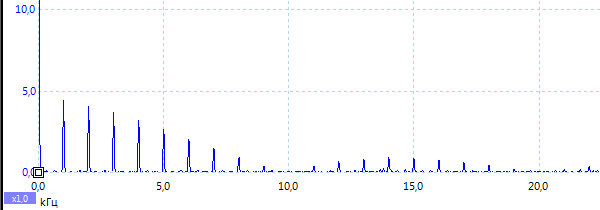
\includegraphics[width=0.45\textwidth]{6.png}&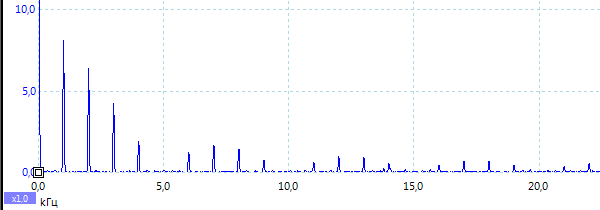
\includegraphics[width=0.45\textwidth]{7a.png}\\
$\nu_{\text{повт}} = 1$ кГц, $\tau = 100$ мкс&$\nu_{\text{повт}} = 1$ кГц, $\tau = 200$ мкс\\
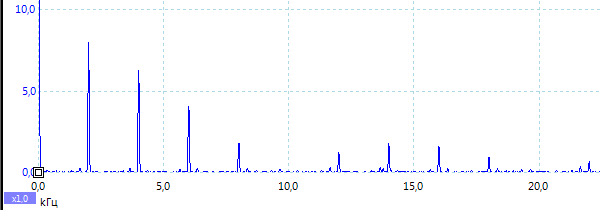
\includegraphics[width=0.45\textwidth]{7b.png}\\
$\nu_{\text{повт}} = 2$ кГц, $\tau = 100$ мкс\\
\end{tabular}
\end{center}
Из данных видно, что, при увеличении $\tau$, уменьшается $\Delta \nu$, а при увеличении $\nu_\text{повт}$, увеличивается расстояние между пиками.

Измерим зависимость $\Delta \nu$ от $\tau$:
\begin{center}
\begin{tabular}{|c|c|c|c|c|}\hline
$\tau\text{, мкс}$&$\nu_0\text{, кГц}$&$\Delta \nu_0\text{, кГц}$&$1/\nu_0\text{, мкс}$&$\Delta 1/\nu_0\text{, мкс}$\\\hline
$40.0$&$30$&$30$&$40.0$&$0$\\\hline
$60.0$&$17$&$17$&$59$&$3$\\\hline
$80.0$&$13$&$13$&$77$&$6$\\\hline
$100.0$&$10$&$10$&$100.0$&$0$\\\hline
$120.0$&$8$&$8$&$125$&$16$\\\hline
$140.0$&$7$&$7$&$140$&$20$\\\hline
$160.0$&$6$&$6$&$170$&$30$\\\hline
$180.0$&$6$&$6$&$170$&$30$\\\hline
$200.0$&$5$&$5$&$200.0$&$0$\\\hline
\end{tabular}\\~\\
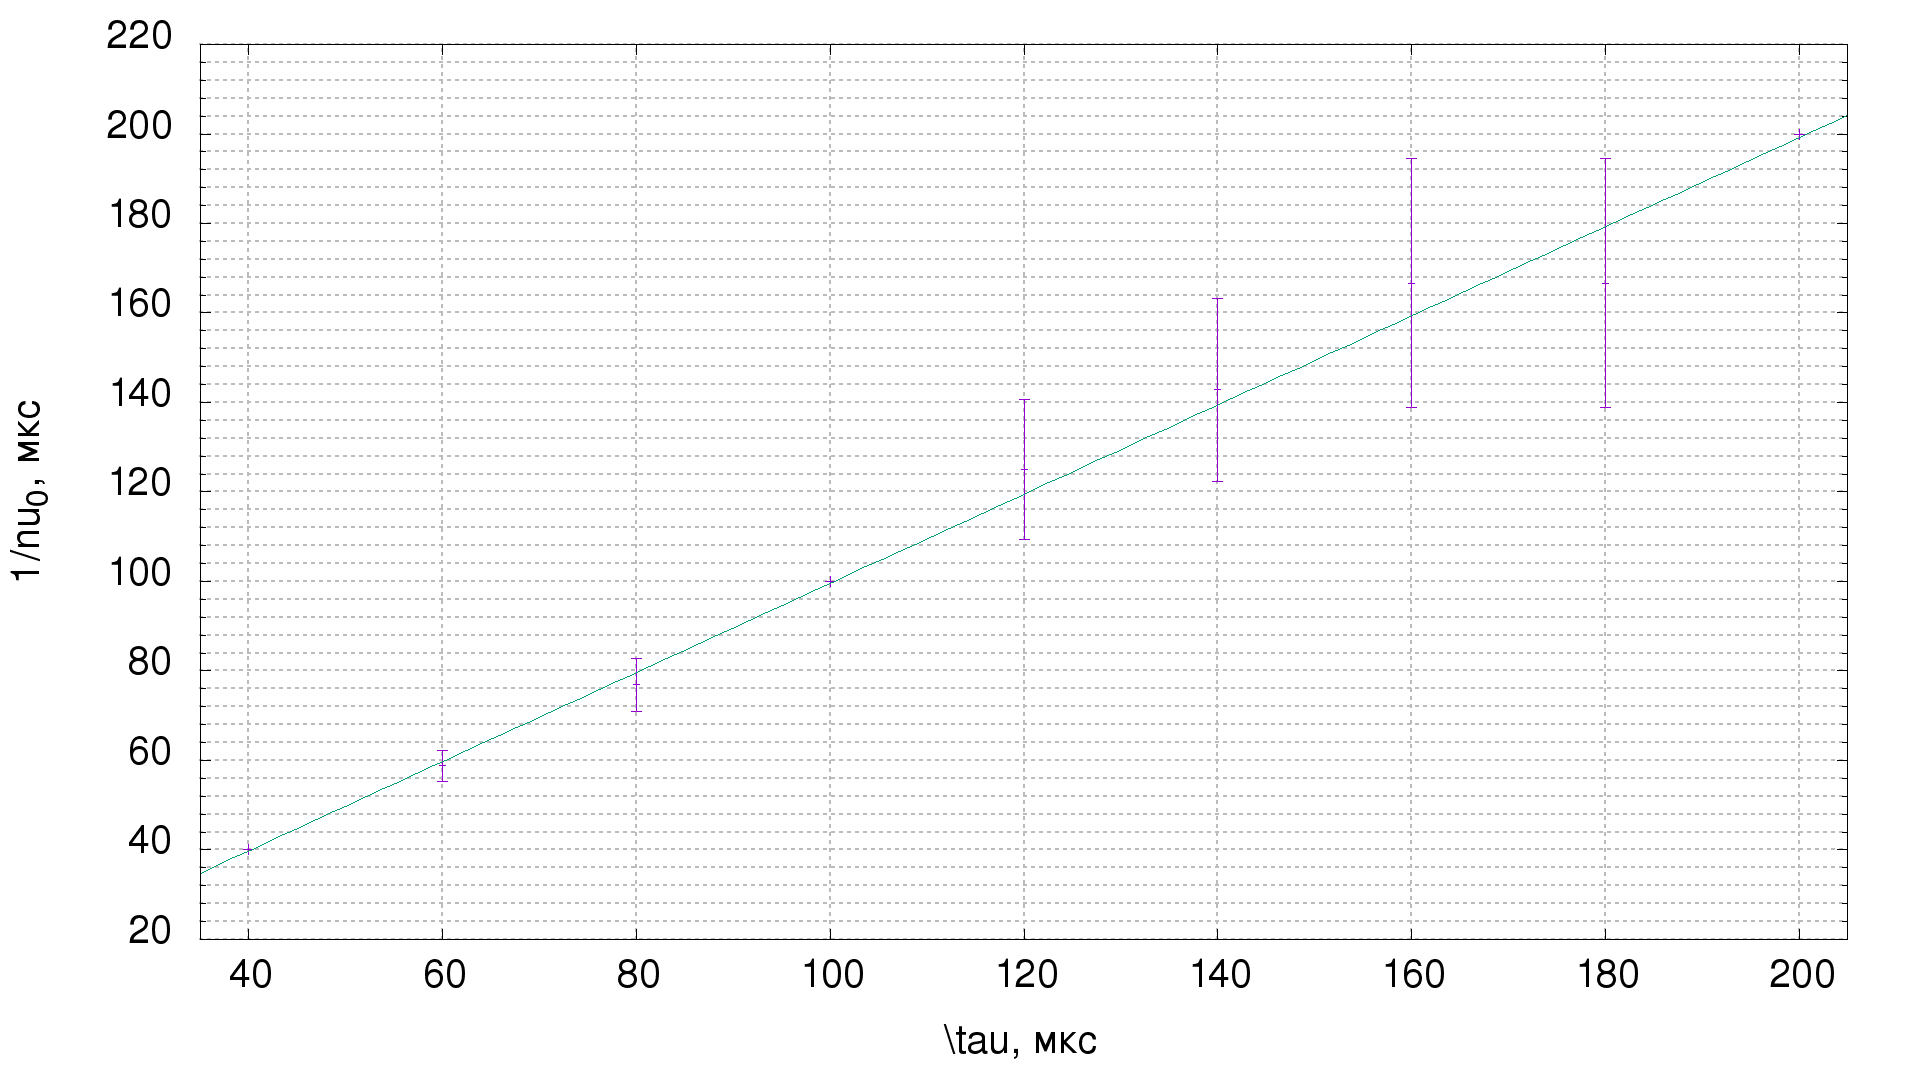
\includegraphics[width=0.95\textwidth]{data.png}
\end{center}

Из графика $\Delta \nu \cdot \tau = 1.004\pm0.014$, что подтверждает соотношение неопределенностей.

\subsection*{Исследование спектра периодической последовательности цугов}
Посмотрим на последовательность цугов с характерными параметрами: $\nu_0 = 50$ кГц частота повторения импульсов $f_\text{повт}=1$ кГц и исследуем спектр этого сигнала для разных длительностей импульса:
\begin{center}
\begin{tabular}{cc}
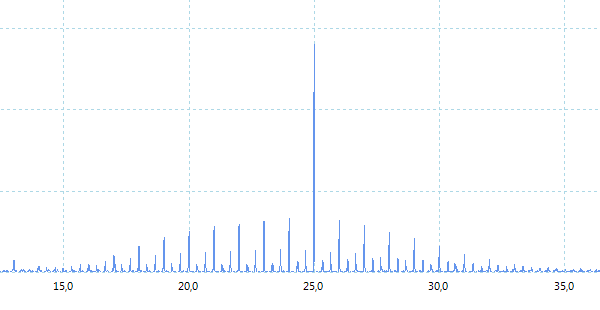
\includegraphics[width=0.45\textwidth]{100_pulse.png}&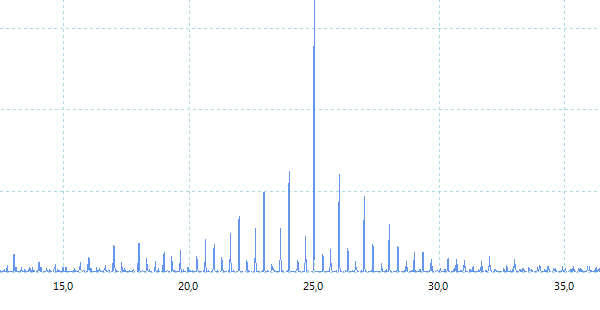
\includegraphics[width=0.45\textwidth]{200_pulse.png}\\
$\tau = 100$ мкс&$\tau = 200$ мкс\\
\end{tabular}
\end{center}
Из данных видно, что при изменении $\tau$ значение $\Delta \omega$ обратнопропорционально меняется.\\

Рассмотрим поведение спектрограммы при фиксировнном значении $\tau$ и меняющемся значении $\nu_0$:
\begin{center}
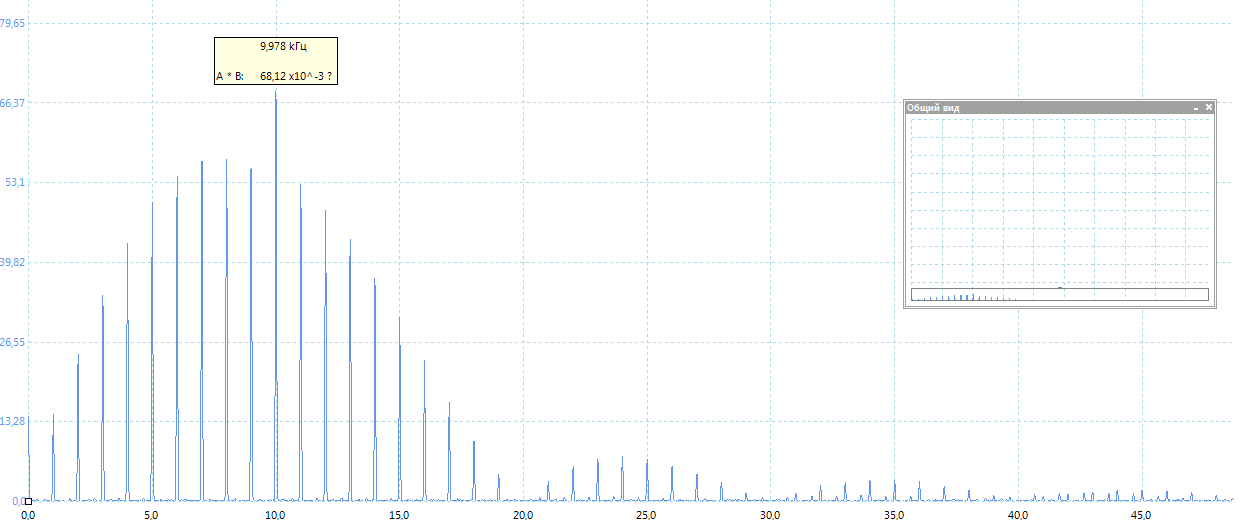
\includegraphics[width=0.95\textwidth]{AB10.png}\\
$\nu_0=10$ кГц
\end{center}
\begin{center}
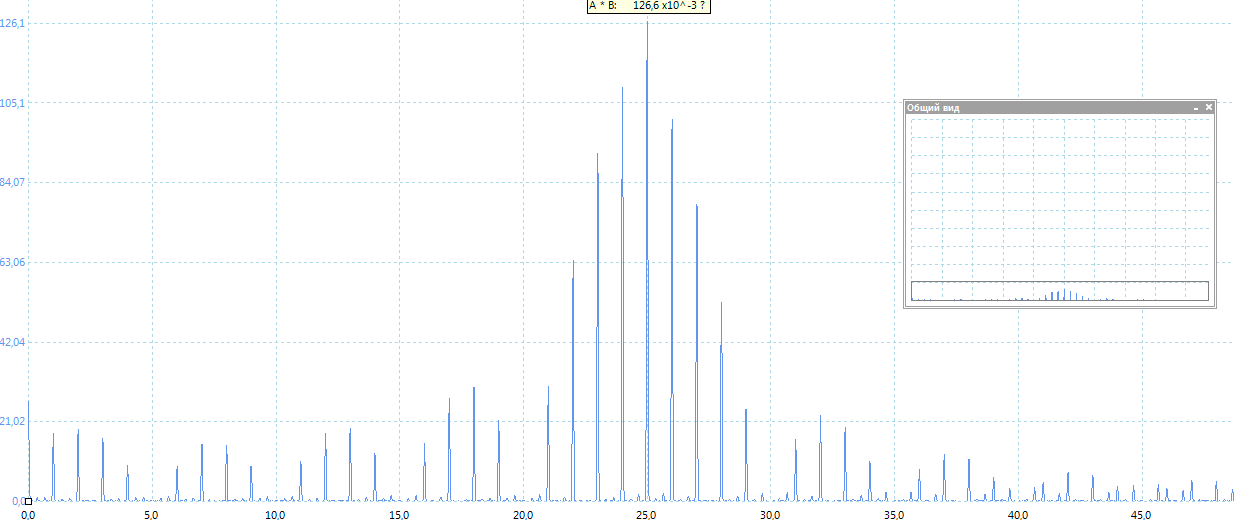
\includegraphics[width=0.95\textwidth]{AB25.png}\\
$\nu_0=25$ кГц
\end{center}
\begin{center}
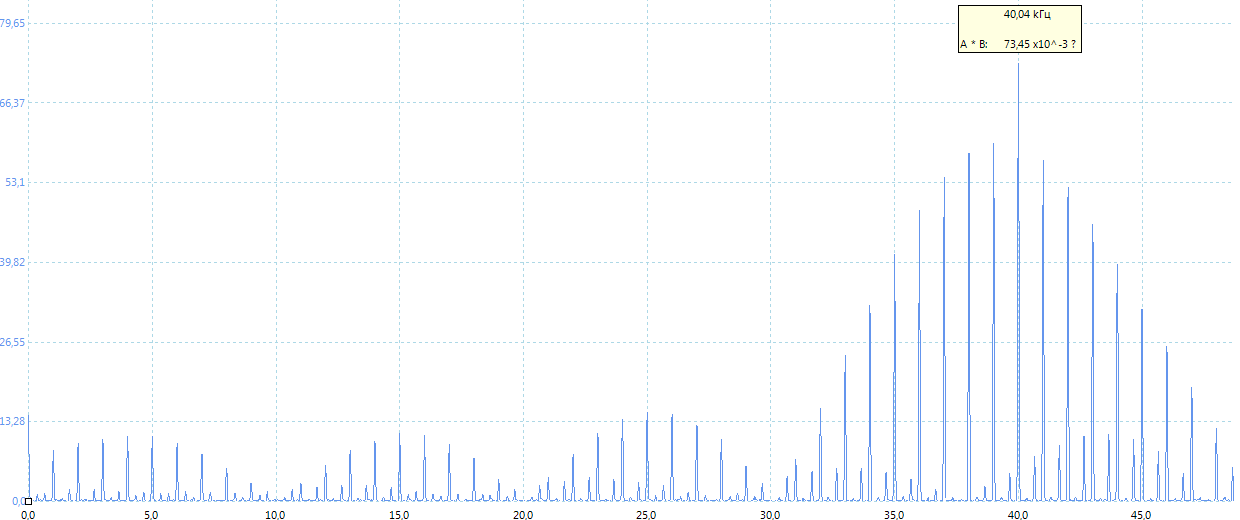
\includegraphics[width=0.95\textwidth]{AB40.png}\\
$\nu_0=40$ кГц
\end{center}
Из данных видно, что при изменении $\nu_0$ картина смещается без изменения расстояния между спектральными компонентами.\\
Рассмотрим то, как это расстояние меняется при изменении $f_\text{повт}$:
\begin{center}
\begin{tabular}{|c|c|}\hline
$f_\text{повт}$&$\nu, \text{кГц}$\\\hline
$0.5$&$0.5$\\\hline
$1.0$&$1.0$\\\hline
$2.0$&$2.0$\\\hline
$4.0$&$4.0$\\\hline
$5.0$&$5.0$\\\hline
\end{tabular}\\~\\
\end{center}
Погрешность результатов определяется погрешностью генератора -- $0.5$ Гц.
$$\frac{f_\text{повт}}{\nu, \text{кГц}} = 1\pm0.1\%,$$
что согласуется с теорией.

\subsection*{Исследование спектра амплитудно модулированного сигнала}
Рассмотрим амплитудно промодулированную синусоиду с параметрами $\nu_0=25$кГц, $\nu_\text{мод}=1$кГц:

\begin{center}
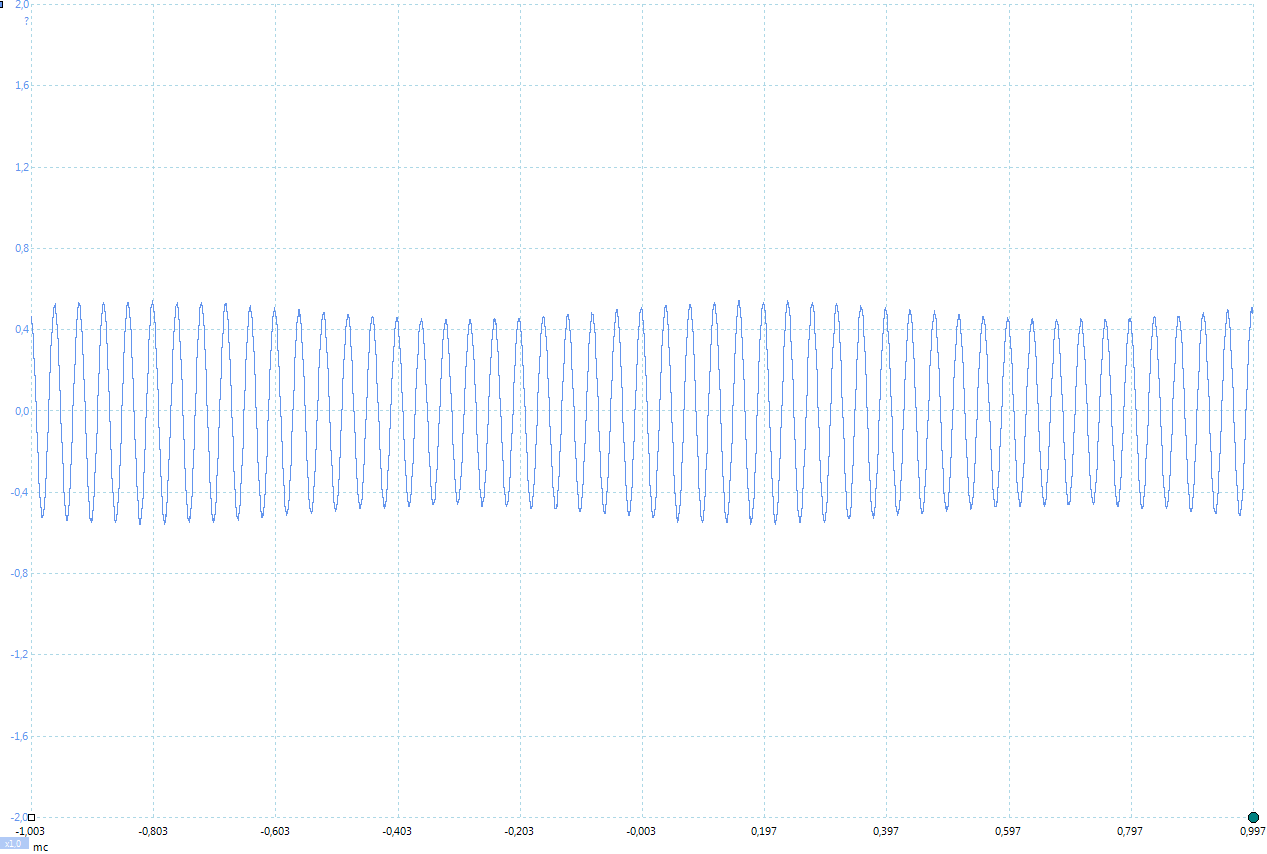
\includegraphics[width=0.95\textwidth]{sin_mod.png}\\
$\nu_0=40$ кГц
\end{center}
\newpage
Посмотрим на спектрограмму этого сигнала:\\
<тут должен быть скрин со спектрограммой, но у меня его нет>
\begin{center}
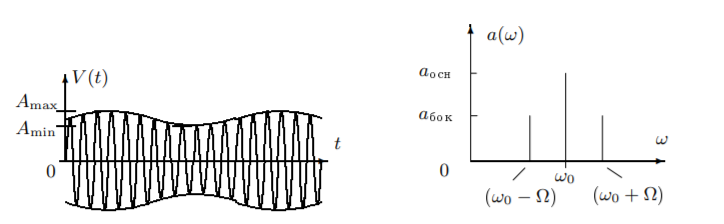
\includegraphics[scale=0.9]{4.png}
\end{center}
Посмотрим зависимость отношения амплитуд $k=A_\text{бок}/A_\text{осн}$ у боковых и остовной частоты от параметра $m = (A_{max} - A_{min}) / (A_{max} + A_{min})$.
\begin{center}
\begin{tabular}{|c|c|c|c|}\hline
$A_{max}-A_{min}\text{, В}$&$A_\text{бок}\text{, В}$&$m$&$k$\\\hline
$0.2$&$0.0160$&$0.1$&$0.0497$\\\hline
$0.6$&$0.0470$&$0.3$&$0.1460$\\\hline
$1.0$&$0.0750$&$0.5$&$0.2329$\\\hline
$1.4$&$0.1070$&$0.7$&$0.3323$\\\hline
$1.8$&$0.1390$&$0.9$&$0.4317$\\\hline
$2.0$&$0.1530$&$1.0$&$0.4752$\\\hline
\end{tabular}\\~\\
$A_\text{осн} = (322\pm0.5)\text{мВ},\,\Delta A_\text{бок}=0.0005\,\text{В},\Delta k=0.0016\,\text{}$
\end{center}
\begin{center}
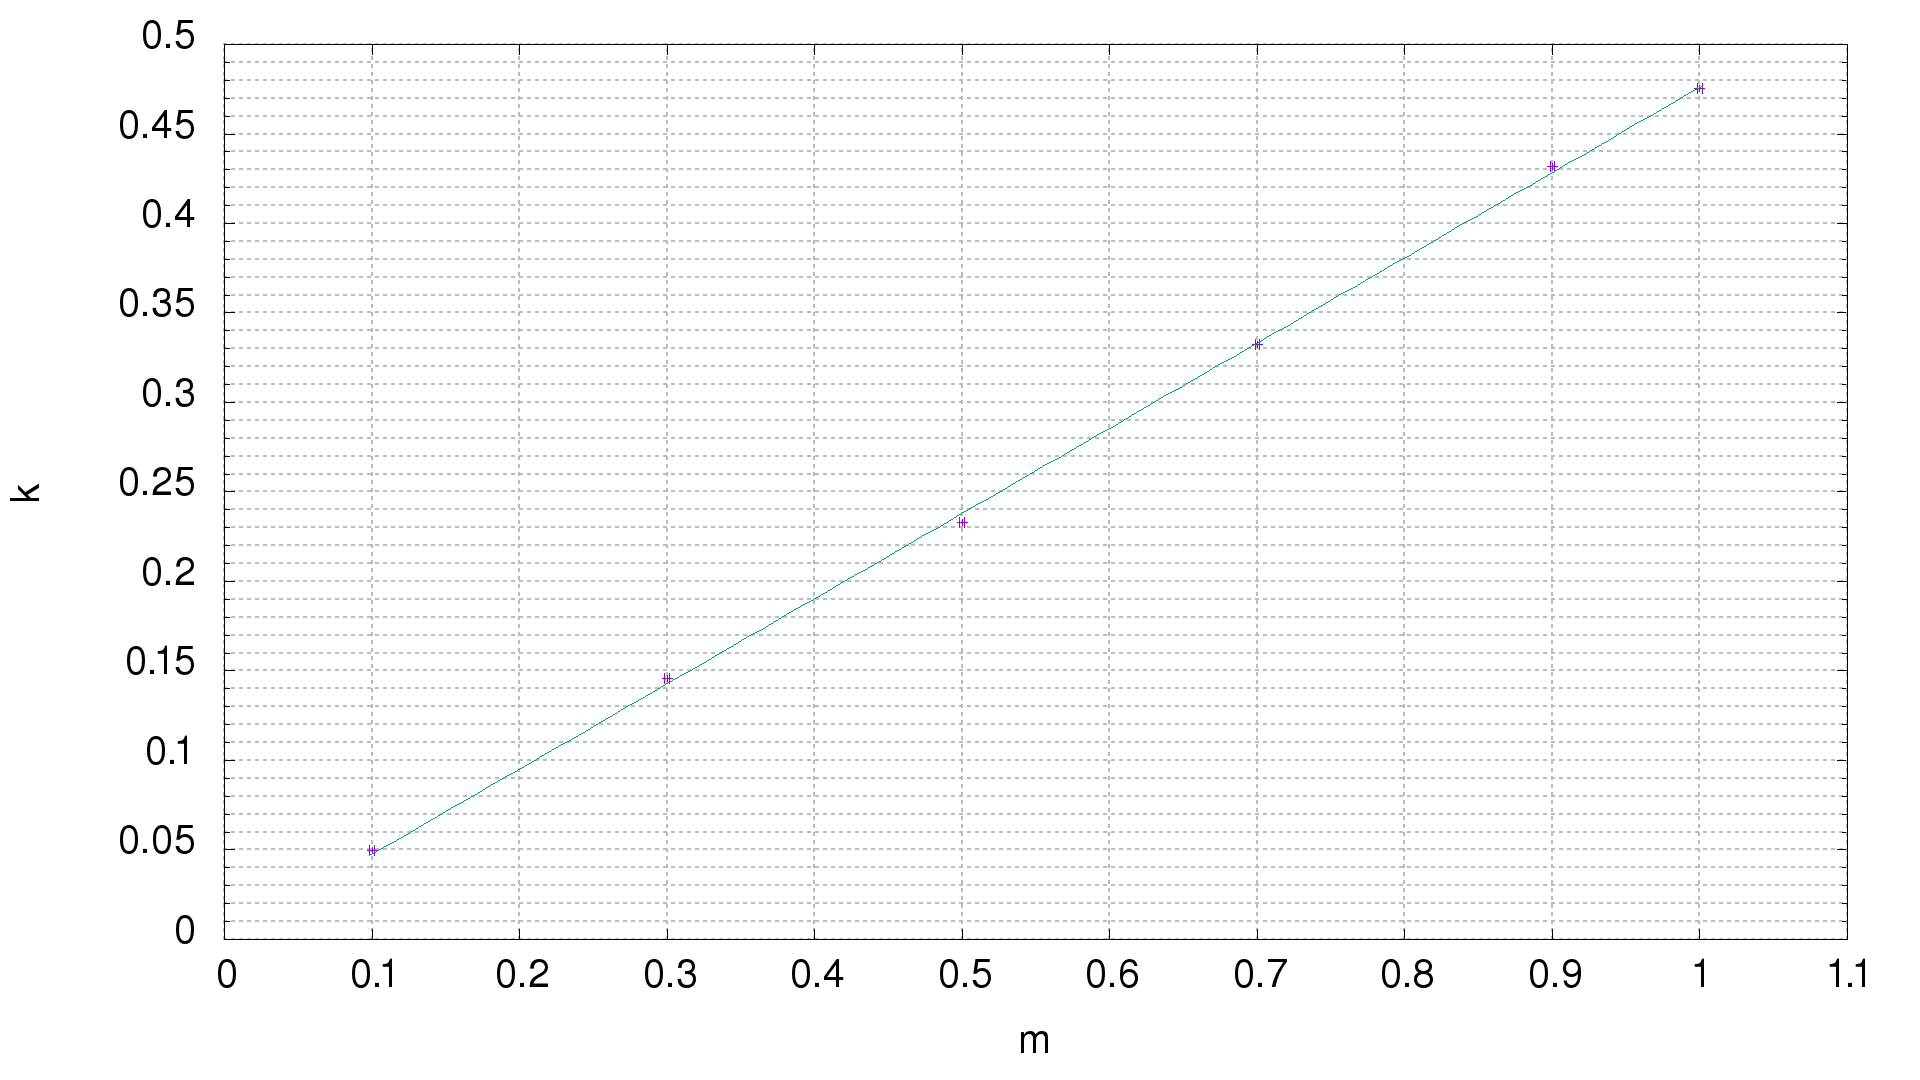
\includegraphics[width=0.95\textwidth]{plot2.png}
\end{center}
Из графика
$$\frac{k}{m} = 0.476\pm0.015,$$
что сходится с теоретическим значением $0.5$.
\section*{Вывод}
В данной работе мы изучили понятие спектра и спектрального анализа, а также исследовали спектральный состав периодических электрических сигналов. 

А именно, мы посмотрели на прямоугольные импульсы, цуги гармонических колебаний, а также гармонические сигналы, модулированные по амплитуде. Кроме того, нами был экспериментально проверен частный случай выполнения соотношения неопределённости. 
  	
\end{document}


125





\lipsum[1-4]
\begin{wrapfigure}{R}{5cm}
\centering
\includegraphics[width=0.20\textwidth]{rd.png}
\caption{1}
\end{wrapfigure}
\lipsum[1-6]


\begin{figure}[h]
\begin{center}$
\begin{array}{cccc}
\includegraphics[width=0.20\textwidth]{rd.png}&
\includegraphics[width=0.20\textwidth]{rd.png}&
\includegraphics[width=0.20\textwidth]{rd.png}&
\includegraphics[width=0.20\textwidth]{rd.png}\\
(1) & (2) & (3) & (4)
\end{array}$
\end{center}
\end{figure}
